Az alkalmazás rendszer szinten mikroszerviz (\ref{sec:mikroszerviz}), a modulok szintjén hexagonális architektúrába (\ref{sec:hexagonalis_architektura}) rendezve készült el. A frontend Angulart (\ref{sec:angular}), a backend és az e-mail kliens Spring Boot-ot (\ref{sec:spring_boot}) használ. A alkalmazáson belüli események kezelésére és tárolására Apache Kafkát (\ref{sec:apache_kafka}) használok.


\section{Mikroszerviz architektúra}\label{sec:mikroszerviz}
Bár a kifejezés már régóta ismert, nincs egy központilag elfogadott, egységes definíció arra nézve, miket nevezünk mikroszervizeknek. A legtöbb szerző jobb híján a visszatérő karakterisztikus tulajdonságuk alapján sorolja be az alkalmazásokat ebbe a kategóriába~\cite{OReally_Microservice_Architecture}. Egy tipikus mikroszerviz a következő tulajdonságoknak felel meg:

\begin{itemize}
	\item	pontosan egy üzleti funkció köré szerveződik,
	\item   más	szervizekkel laza, általában hálózaton keresztül megvalósuló kapcsolatban áll,
	\item   ha szüksége van adatbázisra, akkor sajáttal rendelkezik, más rendszer ezt az adatbázist nem éri el,
	\item	önmagában is működőképes,
	\item	decentralizált, tehát nincs egy a munkáját befolyásoló központi irányítórendszer.
\end{itemize}

A hasonló felépítésükből adódóan, számos olyan eszköz van, ami --  nem kötelezően, de legtöbbször --   együtt fordul elő a mikroszerviz architektúrával. A legfontosabb ilyen fogalmak a:
\begin{description}
	\item[skálázhatóság] a rendszer képessége az áteresztőképességének növelésére.
	Létezik vertikális\footnote{több processzor vagy memória bevonása} és horizontális skálázhatóság\footnote{újabb példányok futtatása}.
	
	\item[konténerizálás] a szerviz futtatása saját elszeparált környezetében hardveres virtualizáció segítsége nélkül.	

	\item[szerviz felderítés] a rendszer által nyújtott szolgáltatások, szervizek automatikus
	felfedezhetősége\footnote{angolul \textit{service discovery}-nek hívják}.
	
	\item[loadbalancer] az a folyamat, ami a bejövő feladatokat erőforrásokhoz rendeli. Legegyszerűbb megvalósítása a \foreignlanguage{british}{\textit{round robin}} algoritmus, célja a terhelés egyforma elosztása.
	
	\item[monitorozás] az önálló szervizek állapotának felügyelése. A monitorozás során nyújtott metrikák kiterjedhetnek a felhasznált memória mennyiségére, processzorigényére, vagy processzeire is.
\end{description}


\section{Hexagonális architektúra}\label{sec:hexagonalis_architektura}
A hexagonális architektúra --  vagy más néven portok és adapterek architektúrája --   egy \foreignlanguage{british}{Alistair Cockburn} által létrehozott \cite{Alistair_Cockburn} szoftverterezési minta. Nevét a cikkben felrajzolt hatszögletű rendszerábrázolásról kapta (\ref{fig:Alistair_Cockburn_hexagonal_architecture} ábra), ami szembemegy a korábban elterjedt réteges elrendezéssel.

Az eredeti szándék mögötte az alkalmazás függetlenítése mindennemű külső függőségtől\footnote{például adatbázis, felhasználók, automatizált tesztek}, így lehetővé téve az üzleti és a technikai igények nagy mértékű szeparálását.
Egy absztrakt port feladata kell legyen a külvilággal való kapcsolat, így az üzleti logika csak az üzenet tartalmáért felelős, az üzenetküldés módjáért már nem.

\begin{figure}[hbt] 
	\centering
	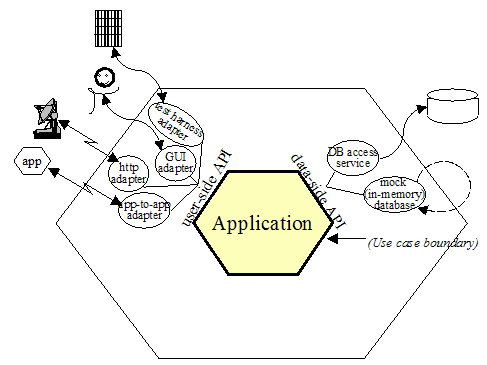
\includegraphics[width=0.85\textwidth]{Alistair_Cockburn_hexagonal_architecture.png}
	\caption[Hexagonális alkalmazások felépítése]{
		A hexagonális alkalmazás külső függőségeinek elszeparálása}
	\label{fig:Alistair_Cockburn_hexagonal_architecture}
	\floatfoot{Forrás: Alistair Cockburn~\cite{Alistair_Cockburn}}
\end{figure}



Ahogy \foreignlanguage{british}{Robert C. Martin} a \foreignlanguage{british}{\textit{The Clean Architecture}} című cikkében \cite{The_Clean_Architecture} összeszedte, a port-adapter és a hasonló architektúrával készülő alkalmazások mind:	
\begin{itemize}
	\item Könnyen, és önmagukban is tesztelhetőek, mivel az üzleti szabályoknak nincs külső függőségük.
	
	\item Függetlenek a külső tényezőktől. Így az alkalmazás által használt felület vagy adatbázis könnyen cserélhető.
	
	\item Keretrendszertől függetlenül is megvalósíthatóak. A megvalósítás nem függ semmilyen könyvtártól vagy egyéb tulajdonságtól.
\end{itemize}
	


\section{Rétegek szeparálása}\label{sec:retegek_szeparalasa}
A hexagonális architektúra (\ref{sec:hexagonalis_architektura} pont) és a hasonló \textit{clean code} \cite{clean_code_chapter_systems} elvek sokszor a különböző szoftver rétegek elkülönítésén alapszanak.


Hogy a feladatok elkülönítése ne vonzza magával az ismétlődő program részletek megnövekedését, célszerű generálni a visszatérő, üzleti funkciót nem hordozó sorokat. Ilyen --  a fordítási időben --   kódot generáló eszköz a Mapstruct és a Lombok.


\section{Konkurencia kezelése}\label{sec:konkurencia_kezekese}
Ha az alkalmazásnak egyszerre több felhasználót kell kiszolgálnia, vagy bármilyen oknál fogva ugyanazt az adatot egy időben több program módosítaná, akkor az inkonzisztens állapot elkerülése érdekében célszerű valamilyen konkurenciakezelési stratégiát alkalmazni. Alapvetően két fajta konkurenciakezelő megoldás létezik:

\begin{description}
	\item[optimista] konkurenciakezelést akkor érdemes használni, mikor számíthatunk arra, hogy az esetek többségében nincs párhuzamos módosítás. Ütközés esetén --  ha egyszerre kellene ugyanazt az adatot módosítani --   a tranzakciót elvetjük és értesítjük a módosítást kezdeményező felet, hogy időközben  az adat megváltozott.
	
	Ez a megoldás tehát nagy mennyiségű adat, és hozzá képest relatív kis számú felhasználó esetén ideális.
	
	\item[pesszimista] konkurenciakezelés esetén, a módosítani kívánt adatot olvasáskor zároljuk, az csak a módosítás befejezése után lesz újra hozzáférhető a többi fél számára.
	
	Az adatok a teljes tranzakció ideje alatt zárolva vannak, ezért ez a megoldás gyakran jár együtt teljesítménycsökkenéssel. A kölcsönös zárolás pedig, --  mikor két vagy több tranzakció egymás befejezésére vár --   könnyen vezethet \textit{deadlock}hoz.
\end{description}


\section{Alkalmazások szeparálása}\label{sec:alkalmazasok_szeparalasa}
Ahogy azt \aref{sec:mikroszerviz}. pontban is írtam, hogy megvalósítható legyen a szervizek laza kapcsolata és egymástól független működése, a mikroszerviz csak a saját adatbázisához férhet hozzá. Ez lehetővé teszi a feladatnak megfelelő adatbázis választását is.

A mikroszervizeken átnyúló üzleti funkciók megvalósítására több megoldás is létezik:
\begin{description}
	\item[API kompozíció] A legegyszerűbben megvalósítható az API kompozíció. Ebben az esetben az applikáció maga végzi el, saját memóriájában az adatok egymáshoz rendelését. 
	
	Kis számú adatnál használható, és célszerű elkerülni hogy az adat kettő vagy annál több számú mikroszervizen keresztül érkezzen meg.
	
	\item[CQRS] A CQRS\footnote{Command Query Responsibility Segregation} az  olvasás és írás műveletének elszeparálásán alapuló megoldás~\cite{OReally_Microservice_Architecture_CQRS}. Lényege hogy a CRUD műveletekről minden esetben egy esemény keletkezik. Ezekre az eseményekre bármelyik mikroszerviz feliratkozhat.
	
	Ha más rendszernek szüksége van az aktuális állapotra, az az események újrajátszásával bármikor megkapható.	
	 
	Az Apache Kafkát (\ref{sec:apache_kafka}) gyakran használják az események kezelésére, mert natívan támogatja az események csoportosítását egyedi azonosító alapján. Beállítható, hogy UUID alapján mindig csak a legfrissebb állapot legyen elérhető, ezzel lecsökkentve a kezdeti olvasáshoz szükséges időt.
		
	\item[Elosztott tranzakciók és Saga] Ha nem csak más szervizek adatainak olvasásáról van szó, hanem több szervizen átívelő, visszagörgethető tranzakciót kell megvalósítani, arra az esetre találták ki a \textit{Saga}-t.
	
	A \textit{Saga} egy hosszú életű elosztott tranzakció~\cite{OReally_Microservice_Architecture_Saga}. A folyamat lépései sorban hajtódnak végre, minden lépés tartalmaz egy utasítást arra az esetre ha vissza kellene görgetni a teljes folyamatot. Ha a folyamat bármelyik lépésnél meghiúsul, onnantól fogva visszafelé minden rendszer egyesével visszaáll a tranzakció előtti állapotra.
\end{description}


\section{Apache Kafka}\label{sec:apache_kafka}
Az Apache Kafka egy üzenet tárolásra és továbbításra kifejlesztett hibatűrő, magas áteresztő képességű, open source alkalmazás~\cite{OReally_Kafka}.

A feladó az üzenetet nem közvetlenül a fogadónak küldi, hanem egy üzenetbrókeren keresztül egy (\textit{topic})-ba teszi közzé. A fogadó fél hogy megkaphassa az üzenetet, feliratkozik az adott témára. 

Redundancia és skálázhatóság miatt egy \textit{topic} több partícióra van elosztva, és ezen felül minden partíció replikálva is van~\cite{OReally_Kafka_Internals}. A partíciók eltérő szerveren lehetnek, ezáltal egy \textit{topic} horizontálisan skálázható. Egy szerver esetleges kiesése esetén a többi szerver át tudja venni a kiesett szerver szerepét.

Az üzenetbrókerek összehangolását a Zookeper szerviz végzi. Mivel minden kafka bróker beregisztrálja magát a szervizbe, a Zookeper mindig naprakész információval rendelkezik az üzenetbrókerekről.

Az üzeneteket Apache Avroval szerializálom. Az Avro lehetővé teszi a kompakt bináris tárolást, de natívan támogatja a JSON reprezentációt is. Az Avrohoz szükséges séma nyilvántartásért és az eltérő verziók kezelésért a Schemaregistry szerver felelős. A kafka kliensek a Schemaregistry szerveren keresztül tudják az üzeneteket olvasni és írni. 



\section{Angular}\label{sec:angular}
Az \foreignlanguage{british}{Angular} egy a \foreignlanguage{british}{Google} által fejlesztett \foreignlanguage{british}{TypeScript} alapú platform és	keretrendszer~\cite{angular_docs}. A segítségével létrehozott kód erősen modularizált, így könnyű vele újra felhasználható és az MVC-elveit követő alkalmazást létrehozni.

Az Angularral készített honlap teljes mértében a kliens oldalon fut, így a szerver oldalon elegendő egy egyszerű, statikus HTML-oldalt visszaadó alkalmazásszerver használata.


\section{Spring Boot}\label{sec:spring_boot}
A \foreignlanguage{british}{Spring Boot} egy a Springre épülő keretrendszer. Mindkét rendszer alapja a függőség befecskendezése\footnote{Angolul \foreignlanguage{british}{\textit{Dependency Injection}}}, ami egy \aref{sec:retegek_szeparalasa} pontban említett tiszta kód \cite{clean_code_chapter_systems} eszköze.

A Spring Boot \cite{introducing_spring_boot} célja hogy gyorsan és egyszerűen lehessen önálló, magas minőségű alkalmazásokat fejleszteni:
\begin{itemize}
	\item az alapbeállítástól való eltérést kell meghatározni\footnote{A Spring Boot dokumentációban ezt röviden \textit{convention over configuration}-nek hívják} ezzel lecsökkentve a konfigurációval töltött időt,
	\item valamint sok gyakran visszatérő problémára\footnote{Például: metrikák, biztonság, adattárolás} nyújt könnyen elérhető megoldást.
\end{itemize}



